%
% Copyright 2017 Markus Borg, Lund University
%
% This work is licensed under a Creative Commons Attribution-ShareAlike 4.0 International License.
% See http://creativecommons.org/licenses/by-sa/4.0/
%
% The dodument is based on a LaTeX template developed by Jean-Philippe Eisenbarth
% https://github.com/jpeisenbarth/SRS-Tex
%
\documentclass{scrreprt}
\usepackage{graphicx}
\usepackage{listings}
\usepackage{underscore}
\usepackage[bookmarks=true]{hyperref}
\usepackage[utf8]{inputenc}
\usepackage[english]{babel}
\hypersetup{
    bookmarks=false,    % show bookmarks bar?
    pdftitle={Software Requirement Specification},    % title
    pdfauthor={Markus Borg},                     % author
    pdfsubject={TeX and LaTeX},                        % subject of the document
    pdfkeywords={TeX, LaTeX, graphics, images}, % list of keywords
    colorlinks=true,       % false: boxed links; true: colored links
    linkcolor=blue,       % color of internal links
    citecolor=black,       % color of links to bibliography
    filecolor=black,        % color of file links
    urlcolor=purple,        % color of external links
    linktoc=page            % only page is linked
}%
\def\myversion{0.1 }
\date{}
%\title
\usepackage{hyperref}
\begin{document}

\begin{flushright}
    \rule{16cm}{5pt}\vskip1cm
    \begin{bfseries}
    	\LARGE{ETSA02-ADM-INS}\\
    	\vspace{1.5cm}
        \Huge{Project\\ Instructions}\\
        \vspace{0.5cm}
        for\\
        \vspace{0.5cm}
        LU Rumble\\
        \vspace{1.5cm}
        \LARGE{Version \myversion approved}\\
        \vspace{1.5cm}
        Prepared by Markus Borg\\
        %\vspace{1.5cm}
        Dept. of Computer Science, Lund University\\
        \vspace{1.5cm}
        \today\\
    \end{bfseries}
\end{flushright}

\tableofcontents


\chapter*{Revision History}

\begin{center}
    \begin{tabular}{|c|c|c|c|}
        \hline
	    Name & Date & Reason For Changes & Version\\
        \hline
	    Markus Borg & 2017-12-07 & Initial draft. & 0.1\\
        \hline
    \end{tabular}
\end{center}

\chapter{Introduction}

\section{Learning goals}
The project primarily aims to increase your ability to develop high quality software systems using established software engineering best practices. Moreover, basic software business concepts will be introduced  as each group will offer their product on a highly competitive market.

The project complements the theoretical concepts introduced during the lectures by taking a practical approach to the presentation of fundamental software engineering concepts such as specification, version control, testing, sprints, and releases. By the end of the course, you will have acquire new skills with essential components of the contemporary  software engineering tool chain: the Java programming language, the Eclipse integrated development environment, the JUnit testing framework, the git configuration management system, GitHub cloud-based project hosting, the Maven build system, and the Checkstyle, PMD, and FindBugs automated quality assurance tools.

On top of your skills with traditional software engineering concepts and the tool chain, you will address aspects of both bespoke and market-driven software engineering. Each group will practice making critical business and engineering decisions in a controlled fashion -- using the course as an open market. The course introduces several important activities in software business, including analyzing the software ecosystem, finding a niche market, marketing a product, competitive pricing strategies, and customer negotiations.

TODO: Make sure this is aligned with the formal course description.

\section{Robocode -- Build the best, destroy the rest!}
The goal of Robocode is to implement the behavior of a robot to compete against other robots in a battle arena. The contestants have no direct influence on the game, instead they write the AI of the robot telling it how to behave and react on events occurring in the battle arena. Battles are running in real-time and on-screen, see Figure~\ref{fig:screenshot}. Robocode battles, referred to as ``rumbles'', are either in the form of duels between individual robots, free-for-all battles with multiple robots, or battles between robot teams.

\begin{figure}
\centering
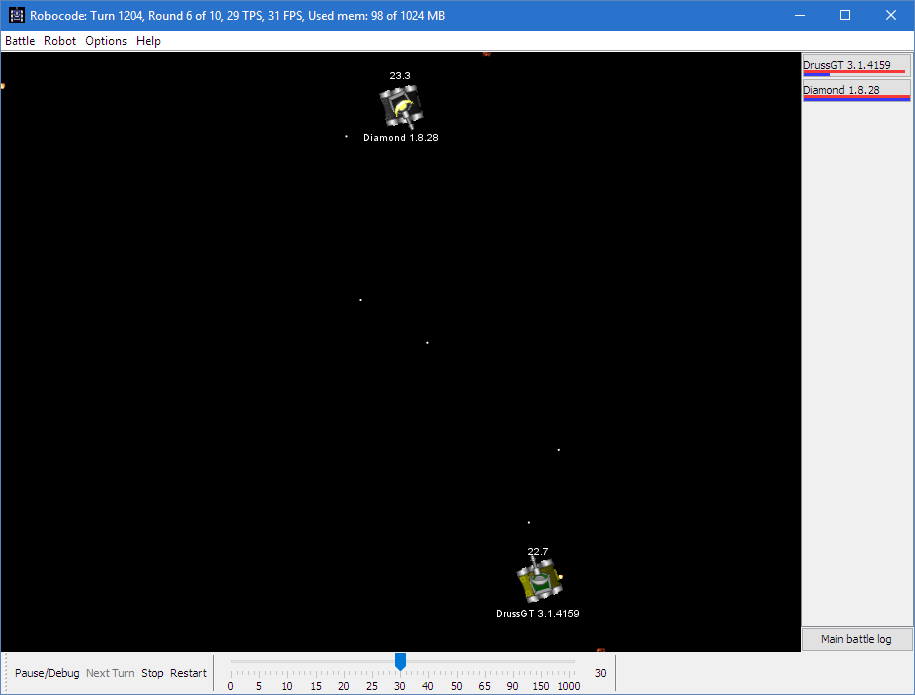
\includegraphics[width=0.80\textwidth]{figures/screenshot.png}
\caption{Screenshot from the Robocode battle arena. (Image credit: robowiki.net user MultiplyByZer0)}
\label{fig:screenshot}
\end{figure}

\textit{From http://robocode.sourceforge.net/docs/ReadMe.html}:
Robocode offers complete development environment, and comes with its own installer, built-in robot editor and Java compiler. Robocode only pre-requires that a JVM (Java Virtual Machine) to exist already on the system where Robocode is going to be installed. Hence, everything a robot developer needs to get started is provided with the main Robocode distribution file (robocode-xxx-setup.jar). Robocode also supports developing robots using external IDEs like Eclipse.

Robocode is an Open Source project, which means that all sources are open to everybody. In addition, Robocode is provided under the terms of EPL (Eclipse Public License). The Robocode game was originally started by Mathew A. Nelson as a personal endeavor in late 2000 and became a professional one when he brought it to IBM in July 2001. In the beginning of 2005, Mathew convinced IBM to release Robocode as Open Source on SourceForge. Eventually, Flemming N. Larsen took over the Robocode project at SourceForge as administrator and developer in July 2006 to continue the original Robocode game -- which now is hosted on GitHub.

\section{Project overview}
Each project team will develop a robot using established software engineering practices. Furthermore, each team will compose a robot team to compete in a ``LU Rumble'' at the final lecture in the course. However, no team is allowed to field their own robot -- instead robots developed by other teams must be purchased on an open market (in truth a somewhat regulated market). Consequently, each team has two primary goals: 1) maximizing profit by selling a successfully engineered robot on the market and 2) winning the LU Rumble by composing a competitive Robocode team. Teams pursue the two goals by completing three main activities that we refer to as \textit{strategizing}, \textit{engineering}, and \textit{monetizing}, respectively.

Figure~\ref{fig:overview} shows the four main phases of the project. First, during the course inception, the course infrastructure and the project tasks are introduce. More importantly, teams consisting of six students (preferably!) are established. Second, the backbone of the course follows: three development sprints mixing engineering, monetizing, and strategizing. Third, purchasers of robots perform acceptance testing to ensure that the delivered robot fulfills the expectations -- otherwise purchasers file business claims to require money back. Fourth, in the last phase of the project, the LU Rumble takes place followed by an awards ceremony to recognize the both winners -- and the most profitable teams.

\begin{figure}
\centering
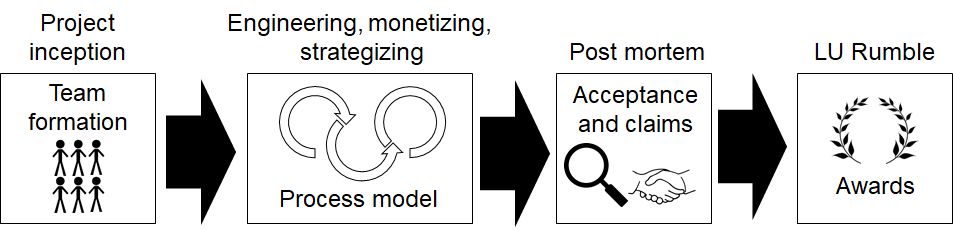
\includegraphics[width=0.99\textwidth]{figures/projectOverview.png}
\caption{Project overview.}
\label{fig:overview}
\end{figure}

The project will be graded as 3, 4, 5 or UG. Project supervisors will in general evaluate the following:
\begin{itemize}
\item The final release meets the final requirements specification. This is partly indicated by the customer's successful acceptance testing.
\item The delivered robot is successful and non-trivial.
\item All the robots behaviors are covered by the requirements specification.
\item The test specification describes a comprehensive verification of the robot. Automated test cases and test reports are provided.
\item The team adhered to the process model and met all deadlines.
\item All deliverables are of high quality.
\end{itemize}

\chapter{Engineering the robot}

\begin{figure}
\centering
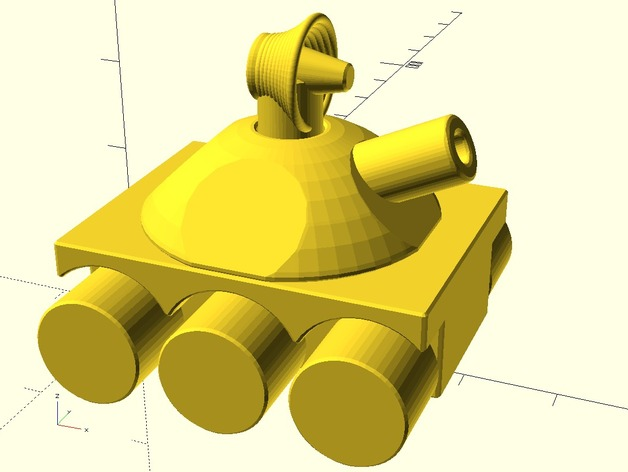
\includegraphics[width=0.50\textwidth]{figures/robotSide.jpg}
\caption{Model of the Robocode robot (\copyright~Klaus Knopper under CC BY-SA 3.0).}
\label{fig:overview}
\end{figure}

\chapter{Monetizing the robot}
After pitching the robot, all teams present a hidden purchase array representing what the team is willing to pay for each of the available robots. For each robot, the highest bidder establishes a customer relationship. If there is a tie, the business relations are assigned randomly.

Signed contracts in grå skåpet.

\chapter{Strategizing to win the LU Rumble}
Learn the domain: http://robocode.sourceforge.net/ and http://robowiki.net/

Purchase a robot from another group. Build a strategy around it. When it has been delivered, complement with other robots. Each team must adhere to two strict constraints: 

\begin{enumerate}
\item Each team must consist of between one and five robots.
\item Each team has a budget of \$100 to purchase robots.
\end{enumerate}

\chapter{Process model}
The process model describing the product development encompasses three sprints, each with a separate set of deliverables. 
After the three sprints, the final part of the course is dedicated to acceptance testing (potentially followed by filing of formal business complaints) and, of course, the concluding LU Rumble and the award ceremonies. 

\begin{figure}
\centering
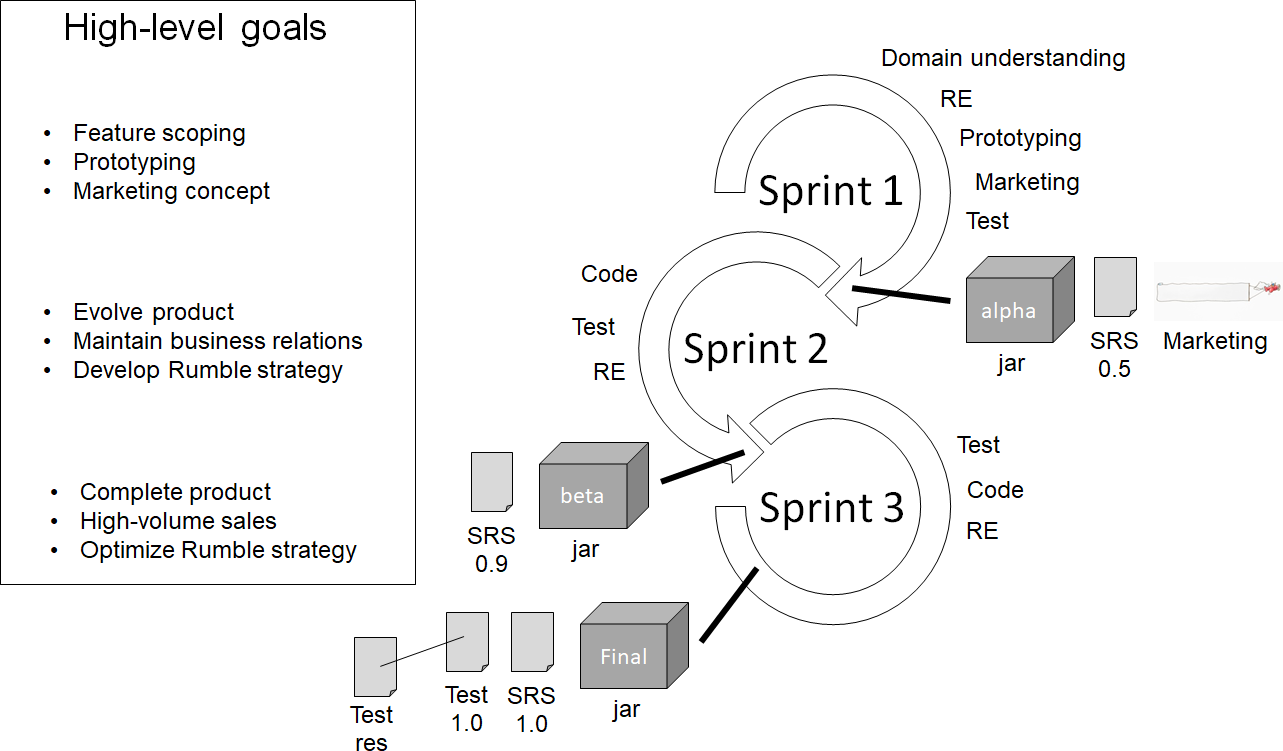
\includegraphics[width=0.85\textwidth]{figures/processModel.png}
\caption{Process model.}
\label{fig:overview}
\end{figure}

%Produktutvecklingen genomförs i fyra faser enligt modellen Unified Software Development
%Process [Jacobson et al., 1999]: 1) Inception, 2) Elaboration, 3) Construction och 4) Transition.
%De mest omfattande faserna är uppdelade i flera iterationer. Faserna visas överst i figur 3.1 och
%iterationerna presenteras nederst.
%
%Varje fas kommer att domineras av en typ av arbete, men även kompletterande arbete av tidigare
%slag, dvs. arbetstyperna överlappar. Exempelvis kommer viss kravhantering att fortsätta ske
%även under fasen Construction – krav kommer troligtvis att behöva kompletteras eller förfinas.
%Varje fas är uppdelad i interationer genom ett antal vecko-sprints. Kombinationen av fasernas
%överlappande arbetsuppgifter samt uppdelning i sprints möjliggör iterativt arbete, vilket ofta är
%en nyckel för framgångsrika utvecklingsprojekt.
%
%Fas 2 och 3 avslutas med milstolpar. Avsikten med en milstolpe är att det tydligt ska framgå
%om den uppnåtts eller inte och på så vis synliggöra hur långt projektet kommit. Exakt vad som
%ingår i de olika milstolparna bör vara känt av samtliga deltagare i projektet och övriga andra
%intressenter, såsom kunder och linjechefer. Projektet har två milstolpar som uppnås när samtliga
%inblandade leverabler är godkända av alla berörda parter. När en milstolpe har passerats
%betraktas huvuddelen av fasens arbete slutfört, därefter sker enbart komplettering och förfining.
%Den grundläggande tanken med projektmodellen är att en fas inte påbörjas förrän föregående 
%milstolpe har uppnåtts. Men även om man inte startar en fas innan de tidigare faserna är
%slutförda är det naturligtvis tillåtet, och i många fall lämpligt, att börja förbereda sig för framtida
%faser. Till exempel, om du vet att du kommer att implementera ett användargränssnitt i
%implementationsfasen men du vet inte hur man gör detta, då du kan börja förbereda implementationsfasen
%tidigt i projektet. Du kan börja studera användargränssnitt, fråga folk som vet mer
%om ämnet eller skapa en mindre prototyp för användargränssnitt bara för att lära sig hur man
%gör. Man kan naturligtvis, i mån av tid, även chansa och påbörja något som man räknar med
%eller hoppas kan bli användbart senare i projektet, men du bör då vara medveten om risken att
%kraven och design kan ändras tidigt i projektet och att det inte är säkert att programkoden du
%har skrivit verkligen blir användbar.

\section{Sprint 1}
Team formation, feature scoping, prototyping, marketing concept

%Projektets första fas innebär en uppstart av projektet. Projektmedlemmarna får en chans att
%träffas och eventuellt nya kontakter etableras. För att gruppen ska fungera bra ihop under projektets
%gång är det viktigt att medlemmarna kommunicerar effektivt med varandra – försök
%komma överens om hur ni kan säkerställa detta. Det är även bra att diskutera era målsättningar,
%eftersom olika förväntningar på arbetsinsats och projektbetyg är en av de främsta orsakerna till
%konflikter i grupparbeten. Relaterat till detta kommer ni även utse olika roller i projektet, dvs.
%ansvarsområden. Detta ska ni beskriva i projektplanen, där ni även i grova drag ska planera
%ert arbete. Slutligen kommer ni att lära känna den dokumentstruktur som ska följas på Google
%Drive.
%Fas 1 avslutas inte med en formell milstolpe, men trots det produceras viktiga resultat:
%Gruppens målsättning förankras
%Infrastruktur skapas på Google Drive
%Projektplan

\section{Sprint 2}
Maintain business relations, evolve product, develop Rumble strategy

%Projektets andra fas innebär en detaljerad analys av kundens behov och en efterföljande teknisk
%kravställning. Arbetet i denna fas utgår från en idé om vad man ska genomföra samt från en
%rad förutsättningar vad gäller tidsplaner, tidsfrister och budget i förhållande till kostnaden. Den
%inledande projektidén är beskriven på en hög nivå som inte är tillräckligt tydlig för att i detalj
%definiera exakt vad som ska utvecklas. Arbetet i denna fas syftar till att precisera exakt vad
%som ska utvecklas under resten av projektet. I denna fas utvecklas även en högnivådesign för
%produkten, dvs. ett klassdiagram.
%Fas 2 avslutas med Milstolpe 1 (MS1). Milstolpen godkänns av projekthandledaren och nås
%när både Projektplan (från Fas 1) och Kravspecifikation är godkända.

\section{Sprint 3}
Complete product, maximize sales, optimize Rumble strategy

%I den tredje fasen av projektet ligger fokus på att utveckla det exekverbara programmet. Detta
%innebär att varje utvecklare utvecklar programkod som kompileras och enhetstestas. Enhetstest
%innebär att man testar delar av programmet isolerat från övriga delar av systemet. Källkoden
%ska även dokumenteras, vilket i kombination med högnivådesignen utgör ett designdokument.
%Utöver detta färdigställs testplan och de testfall som ska genomföras i den sista fasen.
%Fas 3 avslutas med Milstolpe 2 (MS2). Vid denna milstolpe ska Testplan godkännas. Detta
%görs inom projektgruppen efter en intern granskning (se avsnitt 3.6) av dokumentet. När
%testplanen godkänts inom gruppen sätts de i baseline, dvs. version 1.0 varpå de tillsammans
%med granskningsprotokoll skickas för kännedom till projekthandledaren. Om projekthandledaren
%har ytterligare synpunkter kan det bli aktuellt att göra ytterligare förändringar av något eller
%båda dokumenten. För de ändringarna, och eventuell andra framtida ändringar gäller formell
%ändringshantering enligt avsnitt 3.6 med den skillnaden att projekthandledaren inte behöver
%engageras.

\section{Acceptance testing and business claims}
%I den fjärde och sista fasen av projektet ligger fokus på att testa hela systemet och överlämna
%det till kund. Det innebär att alla enheter av programvaran måste integreras till ett system
%Faser och milstolpar 23
%som kan testas. Vid systemtest verifieras att systemet uppfyller alla krav i kravspecifikationen.
%Detta görs genom att man kör samtliga testfall i testplanen. Systemtesterna dokumenteras i en
%Testrapport som för varje testfall visar om det lyckas eller inte. Fasen kan inte avslutas förrän
%alla testfall genomförs utan misslyckanden. Detta innebär att om något test avslöjar fel får man
%gå tillbaka och ändra i de utvecklade produkterna (krav, kod, etc.) och upprepa samtliga testfall.
%Projektgruppen ska även skriva en kort Användarmanual för systemstart.

\section{LU Rumble and Awards}
%Efter fas 4 har den utvecklade produkten levererats till kund och projektet kan därmed avslutas.
%Sedan är det upp till kunden att utföra acceptanstest (se avsnitt 2.5) i syfte att verifiera att det
%som levererats är av tillräcklig kvalitet.

\chapter{Team organization}
Everyone should do everything, but some are more responsible than others.

\begin{itemize}
\item Project manager -- Coordination, time reporting, communication with regulatory body -- Weekly time reports, formal claims (based on failed acceptance test)
\item Development lead -- Design, implementation, source code quality -- jar_v0.5, jar_v0.9, jar_v1.0
\item Test manager -- Test strategy, unit testing, system testing -- Unit tests, Test spec v1.0 (incl. test code), test results
\item Requirements engineer -- End-user perspective, feature scoping, detailed requirements -- SRS v0.5, SRS v0.9, SRS v1.0
\item Sales engineer -- Marketing, customer communication, negotiations -- Marketing concept, signed contract (as supplier)
\item Domain expert -- Mastering Robocode, LU Rumble strategy, supplier communication, negotiations, acceptance testing -- Signed contract (as customer), acceptance test report, team jar-file
\end{itemize}

\chapter{Deliverables}
\begin{itemize}
\item Marketing concepts
\item SRS
\item Source code
\item Releases
\item Test code
\item Test spec
\item Test res
\item Acceptance test
\item LU Rumble team
\end{itemize}

\end{document}
